% !TEX TS-program = knitr
\documentclass{article}\usepackage{graphicx, color}
%% maxwidth is the original width if it is less than linewidth
%% otherwise use linewidth (to make sure the graphics do not exceed the margin)
\makeatletter
\def\maxwidth{ %
  \ifdim\Gin@nat@width>\linewidth
    \linewidth
  \else
    \Gin@nat@width
  \fi
}
\makeatother

\definecolor{fgcolor}{rgb}{0.2, 0.2, 0.2}
\newcommand{\hlnumber}[1]{\textcolor[rgb]{0,0,0}{#1}}%
\newcommand{\hlfunctioncall}[1]{\textcolor[rgb]{0.501960784313725,0,0.329411764705882}{\textbf{#1}}}%
\newcommand{\hlstring}[1]{\textcolor[rgb]{0.6,0.6,1}{#1}}%
\newcommand{\hlkeyword}[1]{\textcolor[rgb]{0,0,0}{\textbf{#1}}}%
\newcommand{\hlargument}[1]{\textcolor[rgb]{0.690196078431373,0.250980392156863,0.0196078431372549}{#1}}%
\newcommand{\hlcomment}[1]{\textcolor[rgb]{0.180392156862745,0.6,0.341176470588235}{#1}}%
\newcommand{\hlroxygencomment}[1]{\textcolor[rgb]{0.43921568627451,0.47843137254902,0.701960784313725}{#1}}%
\newcommand{\hlformalargs}[1]{\textcolor[rgb]{0.690196078431373,0.250980392156863,0.0196078431372549}{#1}}%
\newcommand{\hleqformalargs}[1]{\textcolor[rgb]{0.690196078431373,0.250980392156863,0.0196078431372549}{#1}}%
\newcommand{\hlassignement}[1]{\textcolor[rgb]{0,0,0}{\textbf{#1}}}%
\newcommand{\hlpackage}[1]{\textcolor[rgb]{0.588235294117647,0.709803921568627,0.145098039215686}{#1}}%
\newcommand{\hlslot}[1]{\textit{#1}}%
\newcommand{\hlsymbol}[1]{\textcolor[rgb]{0,0,0}{#1}}%
\newcommand{\hlprompt}[1]{\textcolor[rgb]{0.2,0.2,0.2}{#1}}%

\usepackage{framed}
\makeatletter
\newenvironment{kframe}{%
 \def\at@end@of@kframe{}%
 \ifinner\ifhmode%
  \def\at@end@of@kframe{\end{minipage}}%
  \begin{minipage}{\columnwidth}%
 \fi\fi%
 \def\FrameCommand##1{\hskip\@totalleftmargin \hskip-\fboxsep
 \colorbox{shadecolor}{##1}\hskip-\fboxsep
     % There is no \\@totalrightmargin, so:
     \hskip-\linewidth \hskip-\@totalleftmargin \hskip\columnwidth}%
 \MakeFramed {\advance\hsize-\width
   \@totalleftmargin\z@ \linewidth\hsize
   \@setminipage}}%
 {\par\unskip\endMakeFramed%
 \at@end@of@kframe}
\makeatother

\definecolor{shadecolor}{rgb}{.97, .97, .97}
\definecolor{messagecolor}{rgb}{0, 0, 0}
\definecolor{warningcolor}{rgb}{1, 0, 1}
\definecolor{errorcolor}{rgb}{1, 0, 0}
\newenvironment{knitrout}{}{} % an empty environment to be redefined in TeX

\usepackage{alltt}

\usepackage{amsfonts}
\usepackage{amsmath}
\usepackage{amssymb}
\usepackage{amsthm}
\usepackage{caption}
\usepackage{color}
\usepackage{enumerate}
\usepackage{fancyhdr}
\usepackage{hyperref}
\usepackage{graphicx}
\usepackage{latexsym}
\usepackage{listings}
\usepackage{mathrsfs}
\usepackage{natbib}
\usepackage[nottoc]{tocbibind}
\usepackage{rotating}
\usepackage{url}
\usepackage{mdwlist}

\providecommand{\all}{\ \forall \ }
\providecommand{\bs}{\backslash}
\providecommand{\e}{\varepsilon}
\providecommand{\E}{\ \exists \ }
\providecommand{\lm}[2]{\lim_{#1 \rightarrow #2}}
\providecommand{\m}[1]{\mathbb{#1}}
\providecommand{\nv}{{}^{-1}}
\providecommand{\ov}[1]{\overline{#1}}
\providecommand{\p}{\newpage}
\providecommand{\q}{$\quad$ \newline}
\providecommand{\rt}{\rightarrow}
\providecommand{\Rt}{\Rightarrow}
\providecommand{\vc}[1]{\boldsymbol{#1}}
\providecommand{\wh}[1]{\widehat{#1}}

%\renewcommand\bibname{References}
%\renewcommand{\thesection}{Problem \arabic{section}}
%\renewcommand{\thesubsection}{Part \alph{subsection}}
\numberwithin{equation}{section}

\fancyhead{}
\fancyfoot{}
\fancyhead[R]{\thepage}
\fancyhead[C]{Landau}

\hypersetup{
    colorlinks,
    citecolor=black,
    filecolor=black,
    linkcolor=black,
    urlcolor=blue
}

\definecolor{dkgreen}{rgb}{0,0.6,0}
\definecolor{gray}{rgb}{0.5,0.5,0.5}
\definecolor{mauve}{rgb}{0.58,0,0.82}

\lstset{ 
  language=C,                % the language of the code
  basicstyle=\Large,           % the size of the fonts that are used for the code
  numberstyle= \tiny \color{white},  % the style that is used for the line-numbers
  stepnumber=2,                   % the step between two line-numbers. 
  numbersep=5pt,                  % how far the line-numbers are from the code
  backgroundcolor=\color{white},      % choose the background color. You must add \usepackage{color}
  showspaces=false,               % show spaces adding particular underscores
  showstringspaces=false,         % underline spaces within strings
  showtabs=false,                 % show tabs within strings adding particular underscores
  frame=lrb,                   % adds a frame around the code
  rulecolor=\color{black},        % if not set, the frame-color may be changed on line-breaks within not-black text 
  tabsize=2,                      % sets default tabsize to 2 spaces
  captionpos=t,                   % sets the caption-position 
  breaklines=true,                % sets automatic line breaking
  breakatwhitespace=false,        % sets if automatic breaks should only happen at whitespace
  title=\lstname,                   % show the filename of files included with \lstinputlisting;
  keywordstyle=\color{blue},          % keyword style
  commentstyle=\color{gray},       % comment style
  stringstyle=\color{dkgreen},         % string literal style
  escapeinside={\%*}{*)},            % if you want to add LaTeX within your code
  morekeywords={*, ...},               % if you want to add more keywords to the set
  xleftmargin=0.053in, % left horizontal offset of caption box
  xrightmargin=-.03in % right horizontal offset of caption box
}

\DeclareCaptionFont{white}{\color{white}}
\DeclareCaptionFormat{listing}{\parbox{\textwidth}{\colorbox{gray}{\parbox{\textwidth}{#1#2#3}}\vskip-0.05in}}
\captionsetup[lstlisting]{format = listing, labelfont = white, textfont = white}
% For caption-free listings, comment out the 3 lines above and uncomment the 2 lines below.
% \captionsetup{labelformat = empty, labelsep = none}
% \lstset{frame = single}



\IfFileExists{upquote.sty}{\usepackage{upquote}}{}

\begin{document}
\begin{flushleft}


\Huge
\begin{center}
{\bf STAT 305 D Final Exam}
\end{center} 
\huge
\begin{center}
{\bf Show all your work.}
\end{center}

\normalsize
\begin{enumerate}[1. ]

\item (20 points) Find the following:

\begin{enumerate}[a. ]
\item (4 points) $P((Z - 2, Z + 2) \text{ contains } 0)$, $Z \sim N(0,1)$

{\color{red}
\begin{align*}
P((Z - 2, Z + 2) \text{ contains } 0) &= P(Z - 2 < 0 < Z + 2) \\
&= P(-2 < Z < 2) \\
&= \Phi(2) - \Phi(-2) \\
&= 0.9772 - 0.0227
&= 0.9545
\end{align*}}

\item (4 points) $P((X - 5, X + 5) \text{ contains } 8)$, $X \sim N(3,4)$

{\color{red}
\begin{align*}
P((X - 5, X + 5) \text{ contains } 8) & = P(X - 5 < 8 < X + 5) \\
&= P(X - 13 < 0 < X - 3) \\
&= P(3 < X < 13) \\
&= P(\frac{3 - 3}{2} < \frac{X - 3}{2} < \frac{5 - 3}{2}) \\
&= P(0 < Z < 1) \\
&= \Phi(1) - \Phi(0) \\
&= 0.8413 - 0.5 \\
&= 0.3413
\end{align*}
}

\item (4 points) $P((X - 2, X + 2) \text{ contains } 0)$, $X \sim N(1,0.4)$

{\color{red}
\begin{align*}
P((X - 2, X + 2) \text{ contains } 0) &= P(X - 2 < 0 < X + 2) \\
&= P(-2 < X  < 2) \\
&= P(\frac{-2 -1 }{\sqrt{0.4}} < \frac{X - 1}{\sqrt{0.4}} < \frac{2-1}{\sqrt{0.4}}) \\
&= P(-4.74 < Z < 1.58) \\
&\approx P(Z < 1.58) \\
&= \Phi(1.58) \\
&=  0.9429
\end{align*}
}


\item (4 points) $P((X - 5, X + 5) \text{ contains } 8)$, $X \sim t_7)$

{\color{red}
\begin{align*}
P((X - 5, X + 5) \text{ contains } 8) &= P(X -5 < 8 < X + 5) \\
&= P(3 < X < 13) \\
&= P(t_{7} < 13) - P(t_{7} < 3) \\
&= 1 - 0.099 \\
&= 0.0100
\end{align*}
}


\item (4 points) $P((X - 1.5 \cdot \sigma, X + 1.5 \cdot \sigma) \text{ contains } \mu)$, $X \sim N(\mu,\sigma^2)$

{\color{red}
\begin{align*}
P((X - 1.5 \cdot \sigma, X + 1.5 \cdot \sigma) \text{ contains } \mu) &= P(X - 1.5 \cdot \sigma < \mu < X + 1.5 \cdot \sigma ) \\
&= P(-1.5 < \frac{X - \mu}{\sigma} < 1.5) \\
&= P(-1.5 < Z < 1.5) \\
&= \Phi(1.5) - \Phi(-1.5) \\
&= 0.9331 - 0.0668 \\
&= 0.8664
\end{align*}}


\end{enumerate}


\item (20 points) Every year, your eccentric neighbor carves an excessive number of pumpkins for Halloween and leaves them outside his front door through November. Being eccentric yourself, you weigh all the pumpkins and record their combined weight each year. Here are the data from the last six years: 

\begin{center}
\begin{tabular}{c|cccccc}
Year & 2007 & 2008 & 2009 & 2010 & 2011 & 2012 \\ \hline
Weight (lb) & 311.0 & 271.1 & 320.7 & 274.3 & 332.4 & 304.4   \\ 
\end{tabular}
\end{center}

\begin{enumerate}[a. ]
\item (10 points) Conduct a hypothesis test at $\alpha = 0.05$ to find out if the true mean combined weight of your neighbor's pumpkins exceeds 290 lb.

{\color{red}

First, I calculate the mean weight to be:
\begin{align*}
\ov{x} &= \frac{1}{6} (311.0 + 271.1 + \cdots + 304.4) = 302.3
\intertext{and the standard deviation is:}
s &= \frac{1}{6-1}[(311.0 - 302.3)^2 + (271.1 - 302.3)^2 + \cdots + (304.4 - 302.3)^2] = 24.8
\end{align*}

And here is the hypothesis test:

\begin{enumerate}[1. ]
\item $H_0: \mu = 290$, $H_a: \mu > 290$, where $\mu $ is the true mean combined pumpkin weight.
\item $\alpha = 0.05$
\item I use the test statistic:
\begin{align*}
K = \frac{\ov{x} - 290}{s/\sqrt{n}}
\end{align*}
I assume the combined pumpkin weights are iid $N(\mu, \sigma^2)$. Under the additional assumption that $H_0$ is true, $K \sim t_{n - 1} = t_5$. I will reject $H_0$ if $K > t_{n - 1, 1 - \alpha} = t_{5, 0.95} = 2.02$
\item The moment of truth:
\begin{align*}
K &= \frac{302.3 - 290}{24.8/\sqrt{6}} = 1.21 \\
\end{align*} 
\item With a test statistic of $K =1.21 < 2.02 = t_{n - 1, 1 - \alpha}$, I fail to reject $H_0$. 
\item There is not enough evidence to conclude that your neighbor's true mean combined pumpkin weight (per year) exceeds 290 lb.
\end{enumerate}

}


\item (10 points) Attempt to convince your neighbor of his absurdity by constructing and interpreting a lower 99\% confidence interval for the true mean pumpkin weight.


{\color{red}
Since $n < 25$ and $\sigma^2 $ is unknown, I use the confidence interval:

\begin{align*}
&(\ov{x} - t_{n - 1, \ 1 - \alpha} \cdot \frac{s}{\sqrt{n}}, \ \infty) \\
&= (302.4 - t_{5, 0.995} \cdot{24.8}\sqrt{6}, \ \infty) \\
& = (302.4 - 4.03 \cdot 10.12) \\
&= 261.62
\end{align*}

With 99\% confidence, the true mean annual combined pumpkin weight exceeds 261.62 lb. That's TOO MUCH PUMPKIN MATTER for individual use. 
}

\end{enumerate}


\item (20 points) Not to be outdone, you have been carving and displaying absurd levels of pumpkin matter this entire time. Here are \emph{your} combined pumpkin weights for the last six years.

\begin{center}
\begin{tabular}{c|cccccc}
Year & 2007 & 2008 & 2009 & 2010 & 2011 & 2012 \\ \hline
Weight (lb) & 317.7 & 368.0 & 341.8 & 367.1 & 318.1 & 292.1   \\ 
\end{tabular}
\end{center}

\begin{enumerate}[a. ]
\item (10 points) In a typical year, do you exceed your neighbor in pumpkin weight? Conduct the appropriate hypothesis at $\alpha = 0.05$ to find out.

{\color{red}
First, compute the differences in pumpkin mass


\begin{center}
\begin{tabular}{c|cccccc}
Year & 2007 & 2008 & 2009 & 2010 & 2011 & 2012 \\ \hline
Your pumpkin weight (lb) & 317.7 & 368.0 & 341.8 & 367.1 & 318.1 & 292.1   \\ 
Neighbor's pumpkin weight (lb) & 311.0 & 271.1 & 320.7 & 274.3 & 332.4 & 304.4   \\ 
Difference (lb) & 6.7  & 96.9 & 21.1 & 92.8 & -14.3 & -12.3
\end{tabular}
\end{center}

I compute the mean of the differences (yours - your neighbor's) to be $\ov{d} = 31.8$ and the standard deviation to be $s_d = 50.5$.


Here is the hypothesis test:

\begin{enumerate}[1. ]
\item $H_0: \mu_d = 0$, $H_a: \mu_d > 0$
\item $\alpha = 0.05$
\item I use the test statistic:
\begin{align*}
K = \frac{\ov{d}}{s_d/\sqrt{n}}
\end{align*}
I assume the combined pumpkin weight differences are iid $N(\mu_d, \sigma_d^2)$. Under the additional assumption that $H_0$ is true, $K \sim t_{n - 1} = t_5$. I will reject $H_0$ if $K > t_{n - 1, 1 - \alpha} = t_{5, 0.95} = 2.02$
\item The moment of truth:
\begin{align*}
K &= \frac{31.8}{50.5/\sqrt{6}} = 1.54 \\
\end{align*} 
\item With a test statistic of $K =1.54  < 2.02 = t_{n - 1, 1 - \alpha}$, I fail to reject $H_0$. 
\item There is not enough evidence to conclude that you exceed your neighbor in combined pumpkin weight in a typical year. Your efforts have been in vain. And now you have TOO MANY SEEDS!
\end{enumerate}}

\item (10 points) Construct and interpret a 2-sided 95\% confidence interval for the true mean difference in pumpkin mass between the two of you.

{\color{red}

I use the confidence interval: 

\begin{align*}
&(\ov{d} - t_{n - 1, \ 1 - \alpha/2} \cdot \frac{s_d}{\sqrt{n}}, \ \ov{d} + t_{n - 1, \ 1 - \alpha/2} \cdot \frac{s_d}{\sqrt{n}}) \\
&= (31.8 - t_{5, 0.975} \cdot \frac{50.5}{\sqrt{6}} , \ 31.8 + t_{5, 0.975} \cdot \frac{50.5}{\sqrt{6}} )\\
&= (31.8 - 2.57 \cdot 20.6, 31.8 + 2.57 \cdot  20.6) \\
&= (-21.1, \  84.7)
\end{align*}

I am 95\% confidence interval that the true mean difference between your annual combined pumpkin weight and your neighbor's is between -21.1 lb and 84.7 lb. 
}


\end{enumerate}


\item (20 points) Now that you have bought and carved too many pumpkins, you have too many pumpkin seeds. You also have your neighbor's seeds because he is too eccentric for any kind of seed. You have thousands and thousands of seeds. Naturally, you decide to measure the length of each seed individually, painstakingly, carefully, painstakingly, and individually. Pain! Your 11201 seeds (sample 1) have a mean length of 1.11 cm and a standard deviation of 0.25 cm. Your neighbor's 6732 seeds (sample 2) have a mean length of 1.23 cm and a standard deviation of .25 cm. 

\begin{enumerate}[a. ]
\item (10 points) Use the appropriate hypothesis test at $\alpha = 0.01$ to test the claim that, on average, your seeds are a different length than your neighbor's.

{\color{red}

I will need the pooled standard deviation, $s_p$:

\begin{align*}
s_p &= \frac{(n_1 - 1)s_1^2 + (n_2 - 1) s_2^2}{n_1 + n_2 - 2} \\
&=\frac{(11201- 1)(.25)^2 + (6732 - 1) (.25)^2}{11201 + 6732 - 2} \\
&= 0.25 
\end{align*}


\begin{enumerate}[1. ]
\item $H_0: \mu_1 - \mu_2 = 0$, $H_a: \mu_1 - \mu_2 \ne 0$
\item $\alpha = 0.01$
\item I use the test statistic:
\begin{align*}
K = \frac{\ov{x}_1 - \ov{x}_2}{s_p\sqrt{\frac{1}{n_1} + \frac{1}{n_2}}}
\end{align*}
I assume your pumpkin seed lengths are iid $(\mu_1, \sigma^2)$ and your neighbor's pumpkin seed lengths are iid $(\mu_2, \sigma^2)$. Under the additional assumption that $H_0$ is true, $K \sim N(0,1)$ since the sample sizes are huge. I will reject $H_0$ if $|K| > |z_{1 - \alpha/2}| = z_{ 0.995} = 2.58$
\item The moment of truth:
\begin{align*}
K &=\frac{1.11 - 1.23}{0.25\sqrt{\frac{1}{11201} + \frac{1}{6732}}}  = -31.13 \\
\end{align*} 
\item With $|K| = 31.13 > 2.58$, I reject $H_0$ and conclude $H_a$. 
\item There is overwhelming evidence that your pumpkin seed lengths are different from your neighbor's.
\end{enumerate}



}



\item (10 points) Compute and interpret a two-sided 99\% confidence interval for the difference in true mean pumpkin seed lengths (yours - your neighbor's).


{\color{red}

First I compute:

\begin{align*}
0.25\sqrt{\frac{1}{11201} + \frac{1}{6732}} = 0.00386
\end{align*}

Next, I note that $z_{0.995}$ = 2.58, and the difference in means is 1.11 - 1.23 = 0.12. Now, I compute the confidence interval as

\begin{align*}
&(0.12 - 2.58 \cdot  0.00386, 0.12 + 2.58 \cdot  0.00386) \\
&= (0.11 cm, 0.13 cm)
\end{align*}

With 99\% confidence, your pumpkin seed lengths exceed those of your neighbor by anywhere from 0.11 cm to 0.13 cm.

}



\end{enumerate}





\item (20 points) Return to the New York rivers data:

\begin{center}
\begin{knitrout}
\definecolor{shadecolor}{rgb}{0.969, 0.969, 0.969}\color{fgcolor}\begin{kframe}
\begin{verbatim}
## % latex table generated in R 3.0.0 by xtable 1.7-1 package
## % Fri May 10 12:38:08 2013
## \begin{table}[ht]
## \centering
## \begin{tabular}{rlrrrrr}
##   \hline
##  & Name & X1 & X2 & X3 & X4 & Y \\ 
##   \hline
## 1 & Olean &  26 &  63 & 1.20 & 0.29 & 1.10 \\ 
##   2 & Cassadaga &  29 &  57 & 0.70 & 0.09 & 1.01 \\ 
##   3 & Oatka &  54 &  26 & 1.80 & 0.58 & 1.90 \\ 
##   4 & Neversink &   2 &  84 & 1.90 & 1.98 & 1.00 \\ 
##   5 & Hackensack &   3 &  27 & 29.40 & 3.11 & 1.99 \\ 
##   6 & Wappinger &  19 &  61 & 3.40 & 0.56 & 1.42 \\ 
##   7 & Fishkill &  16 &  60 & 5.60 & 1.11 & 2.04 \\ 
##   8 & Honeoye &  40 &  43 & 1.30 & 0.24 & 1.65 \\ 
##   9 & Susquehanna &  28 &  62 & 1.10 & 0.15 & 1.01 \\ 
##   10 & Chenango &  26 &  60 & 0.90 & 0.23 & 1.21 \\ 
##   11 & Tioughnioga &  26 &  53 & 0.90 & 0.18 & 1.33 \\ 
##   12 & West\_Canada &  15 &  75 & 0.70 & 0.16 & 0.75 \\ 
##   13 & East\_Canada &   6 &  84 & 0.50 & 0.12 & 0.73 \\ 
##   14 & Saranac &   3 &  81 & 0.80 & 0.35 & 0.80 \\ 
##   15 & Ausable &   2 &  89 & 0.70 & 0.35 & 0.76 \\ 
##   16 & Black &   6 &  82 & 0.50 & 0.15 & 0.87 \\ 
##   17 & Schoharie &  22 &  70 & 0.90 & 0.22 & 0.80 \\ 
##   18 & Raquette &   4 &  75 & 0.40 & 0.18 & 0.87 \\ 
##   19 & Oswegatchie &  21 &  56 & 0.50 & 0.13 & 0.66 \\ 
##   20 & Cohocton &  40 &  49 & 1.10 & 0.13 & 1.25 \\ 
##    \hline
## \end{tabular}
## \end{table}
\end{verbatim}
\end{kframe}
\end{knitrout}

\end{center}

Remember:
\begin{itemize}
\item $Y$ is the mean nitrogen content (mg/liter) of the river based on samples based on regular intervals taken in the spring, summer, and fall months.
\item $X1$ is the percentage of surrounding land used in agriculture.
\item $X2$ is the \% surrounding forested land.
\item $X3$ is the \% surrounding residential land.
\item $X4$ is the \% surrounding commercial/industrial land.
\end{itemize}

I fit the model:
\begin{align*}
Y_i = \beta_0 + \beta_1 X_{1, i}  + \beta_2 X_{2, i}  + \beta_3 X_{3, i}  + \beta_4 X_{4, i} + \e_i 
\end{align*}

And here is part of the JMP output:

\begin{center}
\setkeys{Gin}{width=.7\textwidth} 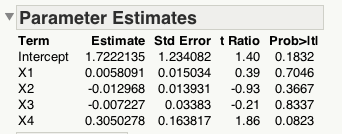
\includegraphics{../../fig/riversparams.png}
\end{center}

\begin{enumerate}[a. ]
\item (4 points) State the assumptions on the $\e_i$'s that we need in order to do inference.

{\color{red} $\e_1, \e_2, \ldots, \e_{20} \sim $ iid $N(0, \sigma^2$). }


\item (4 points) Does \% agricultural land affect the nitrogen content in the rivers? Conduct the appropriate hypothesis test at $\alpha = 0.05$ to find out.

{\color{red}

\begin{enumerate}[1. ]
\item $H_0: \beta_1 = 0$, $H_a: \beta_1 \ne 0$
\item $\alpha = 0.05$
\item I use the test statistic, $K = b_1/ \wh{SD}(b_1)$, which has a $t_{n - p} = t_{20 - 5} = t_{15}$ distribution under $H_0$, along with the assumptions that the model is correct and the error terms behave as in part (a). 
\item The moment of truth: the p-value is already computed in the table as 0.7046.
\item With a p-value $> \alpha$, we fail to reject $H_0$.
\item There is not enough evidence to conclude that river pollution varies with the \% of surrounding land used in agriculture.
\end{enumerate}
}

\item (4 points) Test $H_0: \beta_4 = 0.1$ vs. $H_a: \beta_4 > 0.1$ at $\alpha = 0.01$.


{\color{red}
\begin{enumerate}[1. ]
\item $H_0: \beta_4 = 1$, $H_a: \beta_4 > 1$
\item $\alpha = 0.01$ 
\item I will use the test statistic:
\begin{align*}
K = \frac{b_4 - 0.1}{\wh{SD}(b_4)}
\end{align*}
which has a $t_{15}$ distribution under the assumptions stated in part (b). I will reject $H_0$ if $K > t_{15, 1 - \alpha} = t_{15, 0.99} = 2.60$. 
\item The moment of truth:
\begin{align*}
K = \frac{0.305 - 0.1}{0.164} = 1.25
\end{align*}
\item With $K = 1.25 < 2.60$, we fail to reject $H_0$.
\item There is not enough evidence to conclude that for each percentage increase in commercial/industrial land use, the true mean nitrogen content in the rivers increases by over 0.1 mg/L. In this situation, it doesn't seem that high \% commercial/industrial land is associated with high pollution, although that may be because there is such a low percentage of commercial/industrial land around each river. Also, a small percentage of industrial/commercial land might be enough to catastrophically raise the pollution to a certain level for each river. Also, the covariates are probably highly correlated, which increases the standard errors of the estimates.
\end{enumerate}
}

\item (4 points) Construct and interpret a 2-sided 95\% confidence interval for the intercept in the model.

{\color{red}
In the margin of error, I will use $t_{15, 0.975} = 2.13$. The margin of error is $2.13 \cdot 1.234 = 2.63$. The confidence interval is ($1.72 - 2.63, 1.72 + 2.63$) = $(-0.91, 4.35)$. We're 95\% confident that the true pollution level with no surrounding land used at all is somewhere between -0.91 mg/L and 4.35 mg/L.

}

\item (4 points) What does the model intercept represent? Is there anything problematic in your interpretation on a practical level?
{\color{red}
The intercept represents the pollution level in rivers with no surrounding land at all. But we never observed such rivers: all the rivers in the data had a high degree of developed land. This is a case of extrapolation.
}


\end{enumerate}




\item EXTRA CREDIT (10 points). Suppose I fit a different model with just X2 and X3:

\begin{center}
\setkeys{Gin}{width=.7\textwidth} 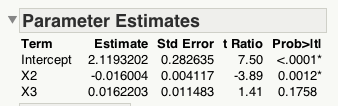
\includegraphics{../../fig/riversparams2.png}
\end{center}

Why is the coefficient on X2 significantly different from 0 here (p-value = 0.0012) even though it was not significantly different from 0 before (p-value = 0.3667)? \q


{\color{red}
The covariates are highly correlated. For example, we expect more residential land when there is also more industrial land. This correlation in the covariates tends to raise the standard errors of the estimated slopes, which decreases the sensitivity of significance tests.
}




\end{enumerate}
\end{flushleft}
\end{document}
